%! TEX root = ../thesis.tex

\chapter{Extensive air showers}
\label{chap:extensive-air-showers}

Extensive air showers describe the particle cascades that are the result of a high-energy cosmic ray interacting with the atmosphere of the earth. While the 
microstate of a given air shower is inherently chaotic, macroscopic variables such as the number of particles in the cascade, its' multiplicity, allow conclusions
on the primary cosmic ray.

In this chapter the various processes which give raise to the jets of energetic particles are discussed. Because hadronic primaries that carry intrinsic 
SU$(3)$-color charges are fundamentally different from leptonic ones which do not, this is done in a two-fold way. The funamental principles kicking off 
electromagnetic cascades are explained in \autoref{sec:heitler-model}. Supplementary information regarding hadronic showers is listed in 
\autoref{sec:heitler-matthews-model}. Finally, the effect of differing hadronic primaries is considered in \autoref{sec:superposition-principle}.

\section{Electromagnetic showers}
\label{sec:heitler-model}

\begin{figure}
	\begin{subfigure}[b]{0.4\textwidth}
		\centering
		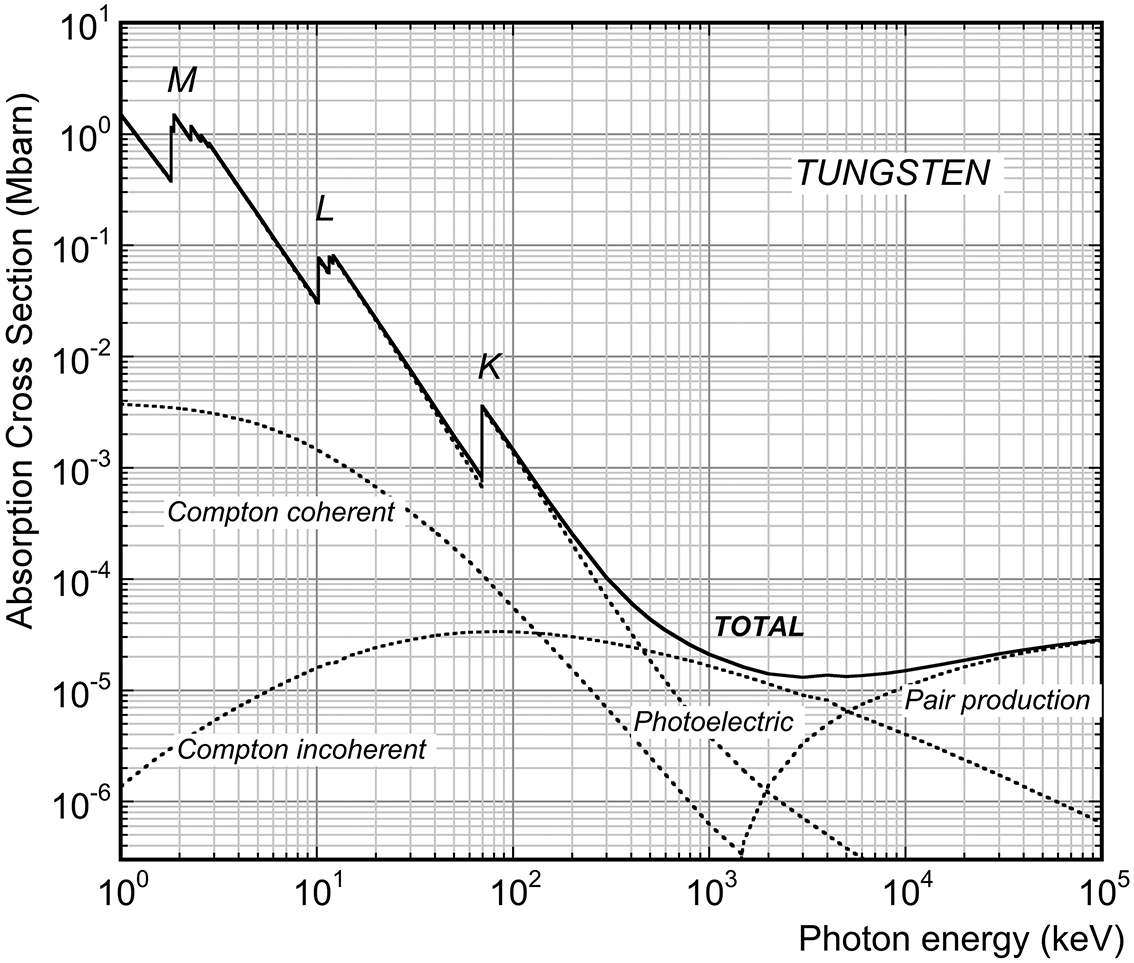
\includegraphics[width=\textwidth]{./plots/photon_cross_section.png}
		\caption{$\mathbf{\gamma}$\textbf{ interactions}}
		\label{fig:gamma-interactions}
	\end{subfigure}
	\hfill
	\begin{subfigure}[b]{0.6\textwidth}
		\centering
		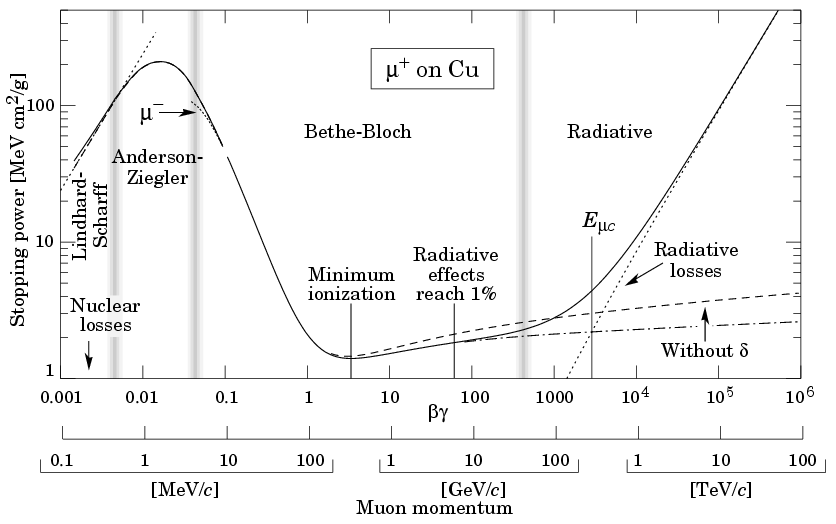
\includegraphics[width=\textwidth]{./plots/electron_ionisation_loss.png}
		\caption{$\mathbf{e^\pm}$\textbf{ interactions}}
		\label{fig:electron-interactions}
	\end{subfigure}
	\caption{\textbf{(a)} Cross section for different energy loss processes of a photon in tungsten. The sudden spikes correspond to the transition energy of 
	increasingly higher-energy electron shells. From \cite{chen2007interactions}. \textbf{(b)} Stopping power of copper, representatively on an antimuon $\upmu^+$, 
	with respect to its' momentum. Plot adopted with changes from \cite{meroli2017straggling}.}
	\label{fig:ionization-losses}
\end{figure}

The dominating interaction of $E > \SI{10}{\mega\electronvolt}$ photons in matter is $e^+e^-$ pair production, whereas for electrons/positrons the creation of a
$\gamma$ via Bremsstrahlung prevails at high energies. This is shown in \autoref{fig:ionization-losses}. Consequently, an entire cascade of $e^\pm$ and photons can
emerge from a single primary particle, as realised by Heitler in \cite{heitler1984quantum}. 

Of particular interest in these showers are, apart from the primary particles energy $E_0$ and arrival direction $(\theta, \phi)$, the atmospheric depth 
$X_\text{max}$ at which it reaches its' maximum multiplicity, as well as the \textbf{L}ateral \textbf{D}istribution \textbf{F}unction (LDF), that parametrizes the 
distribution of particles along the shower axis. An important variable that influences both values is the radiation length $X_0$. It represents the characteristic
length at which an $e^\pm$ loses $1-\frac{1}{e}\approx63\%$ of its energy. It also corresponds to the mean free path of a photon in matter up to a factor $7 / 9$ 
\cite{gupta2010calculation}. Neglecting said factor and assuming that new particles on average inherit half of the parent energy, describing the multitude of 
particles contained in an electromagnetic shower becomes a counting exercise in the context of the Heitler-model.

With each radiation length, the number of particles $N$ in the shower double, while the energy per particle, $E_\text{pp}$, halves. After traversing an atmospheric 
depth of $n\cdot X_\text{max}$, typically measured in units of \SI{}{\gram\per\centi\meter\squared}, they consequently read

\begin{equation}
\label{eq:heitler-parameters}
N(n) = 2^n, \qquad E(n) = \frac{E_0}{2^n}.
\end{equation}

After sufficient interactions, the energy of each individual particle $E_\text{PP}$ will have degraded to such an extent that other processes are no longer 
negligible compared to Bremsstrahlung and pair production. This occurs at the critical energy $E_{c,\,\text{EM}}$ below which the shower rapidly stops creating new particles and
dies out as a result. It follows via \autoref{eq:x-max} and \ref{eq:n-max} that both $X_\text{max}$ as well as $N_\text{max}$ increase with $E_0$. The multiplicity 
arising from these assumptions alongside a stylized propagation of the thus created shower is represented in \autoref{fig:heitler-model}. 

\begin{align*}
E_\text{PP}\,(n_\text{max}) &\stackrel{!}{=} E_c \stackrel{\eqref{eq:heitler-parameters}}{=} \frac{E_0}{2^{n_\text{max}}}\\
\Leftrightarrow \qquad \qquad n_\text{max} &= \left\lfloor \log_2 \left( \frac{E_0}{E_{c,\,\text{EM}}} \right) \right\rfloor \\[7pt]
\Rightarrow \qquad \qquad\!\! X_\text{max} &= n_\text{max}\cdot X_0 = \left\lfloor \log_2 \left( \frac{E_0}{E_{c,\,\text{EM}}} \right) \right\rfloor. \numberthis\label{eq:x-max} \\
\Rightarrow \qquad \qquad\!\! N_\text{max} &= 2^{n_\text{max}} = \left\lfloor \frac{E_0}{E_{c,\,\text{EM}}} \right\rfloor. \numberthis\label{eq:n-max}
\end{align*}

\begin{figure}
	\centering
	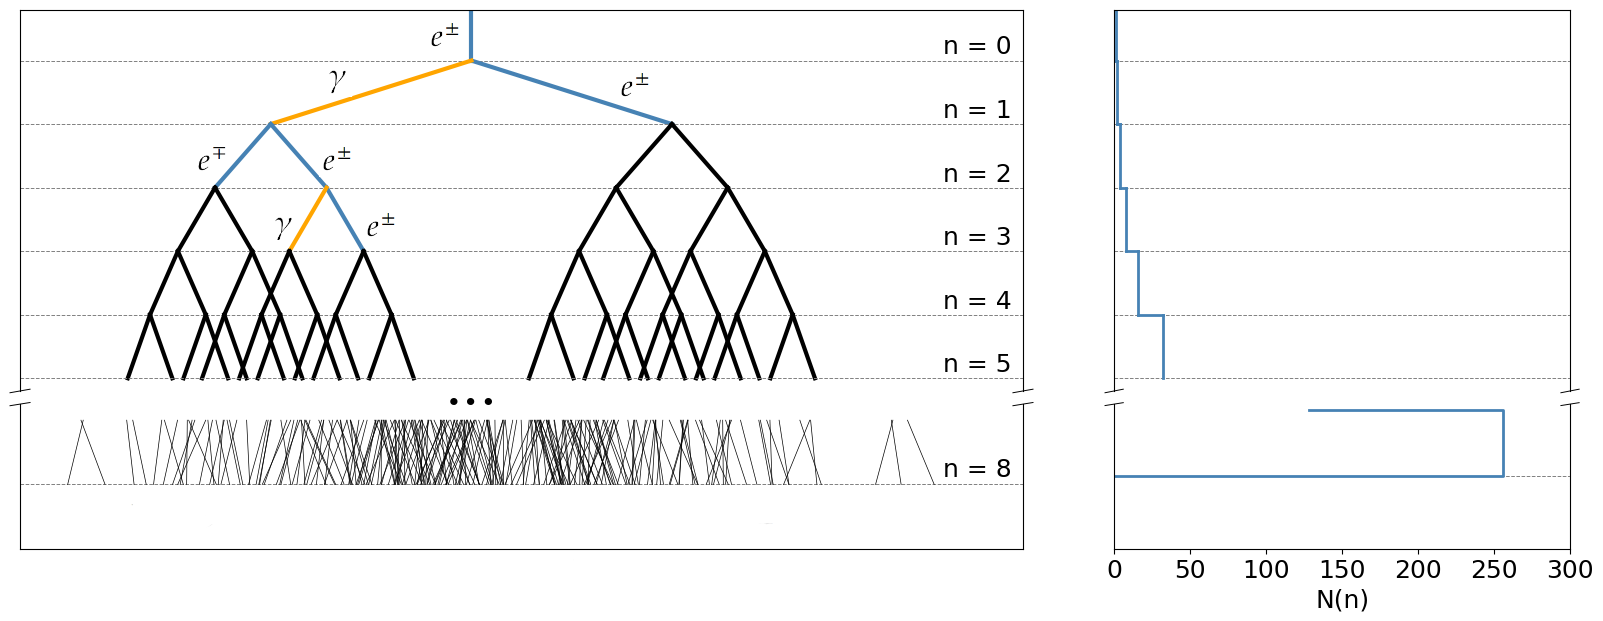
\includegraphics[width=\textwidth]{./imgs/heitler_shower.png}
	\caption{Shown on the left is the stylized propagation of an extensive air shower through the atmosphere according to the Heitler-model, quantized in units
	of $X_0$. The energy of the primary particle is of order $2^8\cdot E_{c,\,\text{EM}}$, which allows for 8 bifurcation steps, and $N_\text{max}=256$ shower particles. The
	multiplicity of the shower after each step is shown in the right subplot.}
	\label{fig:heitler-model}
\end{figure}

The number of particles at a given distance from the shower axis (y-axis in \autoref{fig:heitler-model}) is essentially random, but follows a statistical basis,
the lateral distribution function. The LDF can either be derived approximately from first principles \cite{kamata1958lateral} or empirically, as is done in 
\cite{greisen1960cosmic}. The latter arrives at a closed form approximation for the local density $\rho$ of particles given a shower with multiplicity $N$ at a 
distance $r$ from the shower axis as

\begin{equation}
\label{eq:NKG-electrons}
\rho_\text{EM}(N, r)=\frac{0.4\,N}{r_\text{M}^2} \left(\frac{r_\text{M}}{r}\right)^{0.75} \left(\frac{r_\text{M}}{r+r_\text{M}}\right)^{3.25}\left(1+\frac{r}{11.4\,r_\text{M}} \right).
\end{equation}

In \autoref{eq:NKG-electrons}, the Molière radius $r_\text{M}$ characterizes the lateral spread in multiple scattering processes. It is of order 
$r_\text{M}\approx\SI{100}{\meter}$ for interactions that are relevant here, and in general depends on the density of the considered material 
\cite{moliere1947theorie}.

\section{Hadronic showers}
\label{sec:heitler-matthews-model}

Hadronic primaries will readly produce color-charged secondaries, as has been shown many times in particle accelerators. In order to model the development of 
hadronic showers, the model discussed in \autoref{eq:heitler-parameters} thus needs to be adjusted. An example theory has been developed by Matthews in 2005. 
Following the reasoning in \cite{matthews2005heitler}, after traversing an atmospheric depth corresponding to the hadronic interaction length, a proton creates on 
average $N_\pi \approx 15$ pions, of which two thirds are charged, and one third is uncharged. The corresponding decay channels of the light $\pi$-mesons with the 
largest \textbf{B}ranching \textbf{R}atios (BR) are 

\begin{align*}
	\pi^{+} &\rightarrow \upmu^{+} + \nu_\upmu \!\!\!  \qquad\qquad (\text{BR}\approx0.9999,\,\tau=\SI{2.6033e-8}{\second} \; \text{\cite{PDG}}), \\
	\pi^{-} &\rightarrow \upmu + \bar{\nu}_\upmu \qquad\qquad (\text{BR}\approx0.9999,\,\tau=\SI{2.6033e-8}{\second} \; \text{\cite{PDG}}), \\
	\pi^0 &\rightarrow 2\gamma \!\! \qquad\qquad\qquad (\text{BR}\approx0.9882,\,\tau=\SI{8.5e-17}{\second}\; \text{\cite{PDG}}).
\end{align*}

With a mean lifetime of just attoseconds, the $\pi^0$ decay instantly before being able to continue the cascade process. In this fashion, the uncharged particles 
initiate a Heitler shower such as the one in \autoref{sec:heitler-model}, by providing high-energy photons. It follows that every hadronic shower has an 
electromagnetic component. Moreover, assuming that the inherited energy from the parent particle is roughly uniformly distributed among its' children, one third of
the remaining energy in the hadronic component is lost to the electromagnetic component per hadronic interaction length. 

Meanwhile, the charged pions repeat the procedure of creating secondary mesons, kicking off the hadronic component of the shower in the process.

Similar to the reasoning in \autoref{sec:heitler-model}, a primary of given energy initiates a shower of a specific multiplicity $N_\text{max}$. This is reached 
after $n_\text{max}$ steps, where the energy per particle $E_\text{PP}(n_\text{max})$ is below the critical energy $E_{c,\,\text{had.}}$ at which the mesons ionize rather than 
continue the cascade. After this last step, the charged pions eventually decay into muons and neutrinos. The shower characteristics are thus given by

\begin{equation}
N_\text{had}(n) = \left(\frac{2\,N_\pi}{3}\right)^n,\qquad E_\text{PP}(n) = \frac{E_0}{N_\pi^n},\qquad n_\text{max}=\left\lfloor\log_N\left(\frac{E_0}{E_{c,\,\text{had}}}\right)\right\rfloor,
\end{equation}

wheras the maximum multiplicity (ignoring neutrinos) in the shower is calculated as

\begin{equation}
\label{eq:n-max-matthews}
N_{\text{max},\,1} = \underbrace{ \frac{3}{2}\left( \frac{2}{3}N_\pi\right)^{n_\text{max}}  }_\text{Muon component} + \;\; 
		     \underbrace{\sum\limits_{k = 1}^{n_\text{max}-1} \frac{N(k)}{3} \cdot \left\lfloor 
		     \frac{E_\text{PP}(k) }{E_{c,\,\text{EM}}}\right\rfloor}_\text{EM component}.
\end{equation}

The muons stemming from pion decay follow a different LDF than the electromagnetic component. Again following the analysis in \cite{greisen1960cosmic}, the muonic
LDF can be recovered as

\begin{equation}
\label{eq:NKG-muons}
\rho_\upmu(N, t) = 18\,\left(\frac{N}{10^6 \cdot r}\right)^\frac{3}{4} \cdot \;\,\left(1 + \frac{r}{320}\right)^{-\frac{5}{2}}.
\end{equation}

While the above \autoref{eq:NKG-muons} drops off slower $\mathcal{O}(r^{-\frac{3}{2}})$ compared to the electromagnetic component ($\mathcal{O}(r^{-3})$), the
immediate vicinity of the shower axis contains mostly photons and leptons from the EM subshower. Further out, the muonic component takes over. This is visualized
in \autoref{fig:component-LDF}. Due to this reason, and the fact that muons can carry considerable amounts of energy faraway from the shower axis, the muonic 
footprint of a shower often appears much more "patchy" compared to the EM portion. This knowledge is espically useful when distinguishing between hadron- and 
photon-induced air showers (compare \cite{capistran2015new}).

\begin{figure}
	\centering
	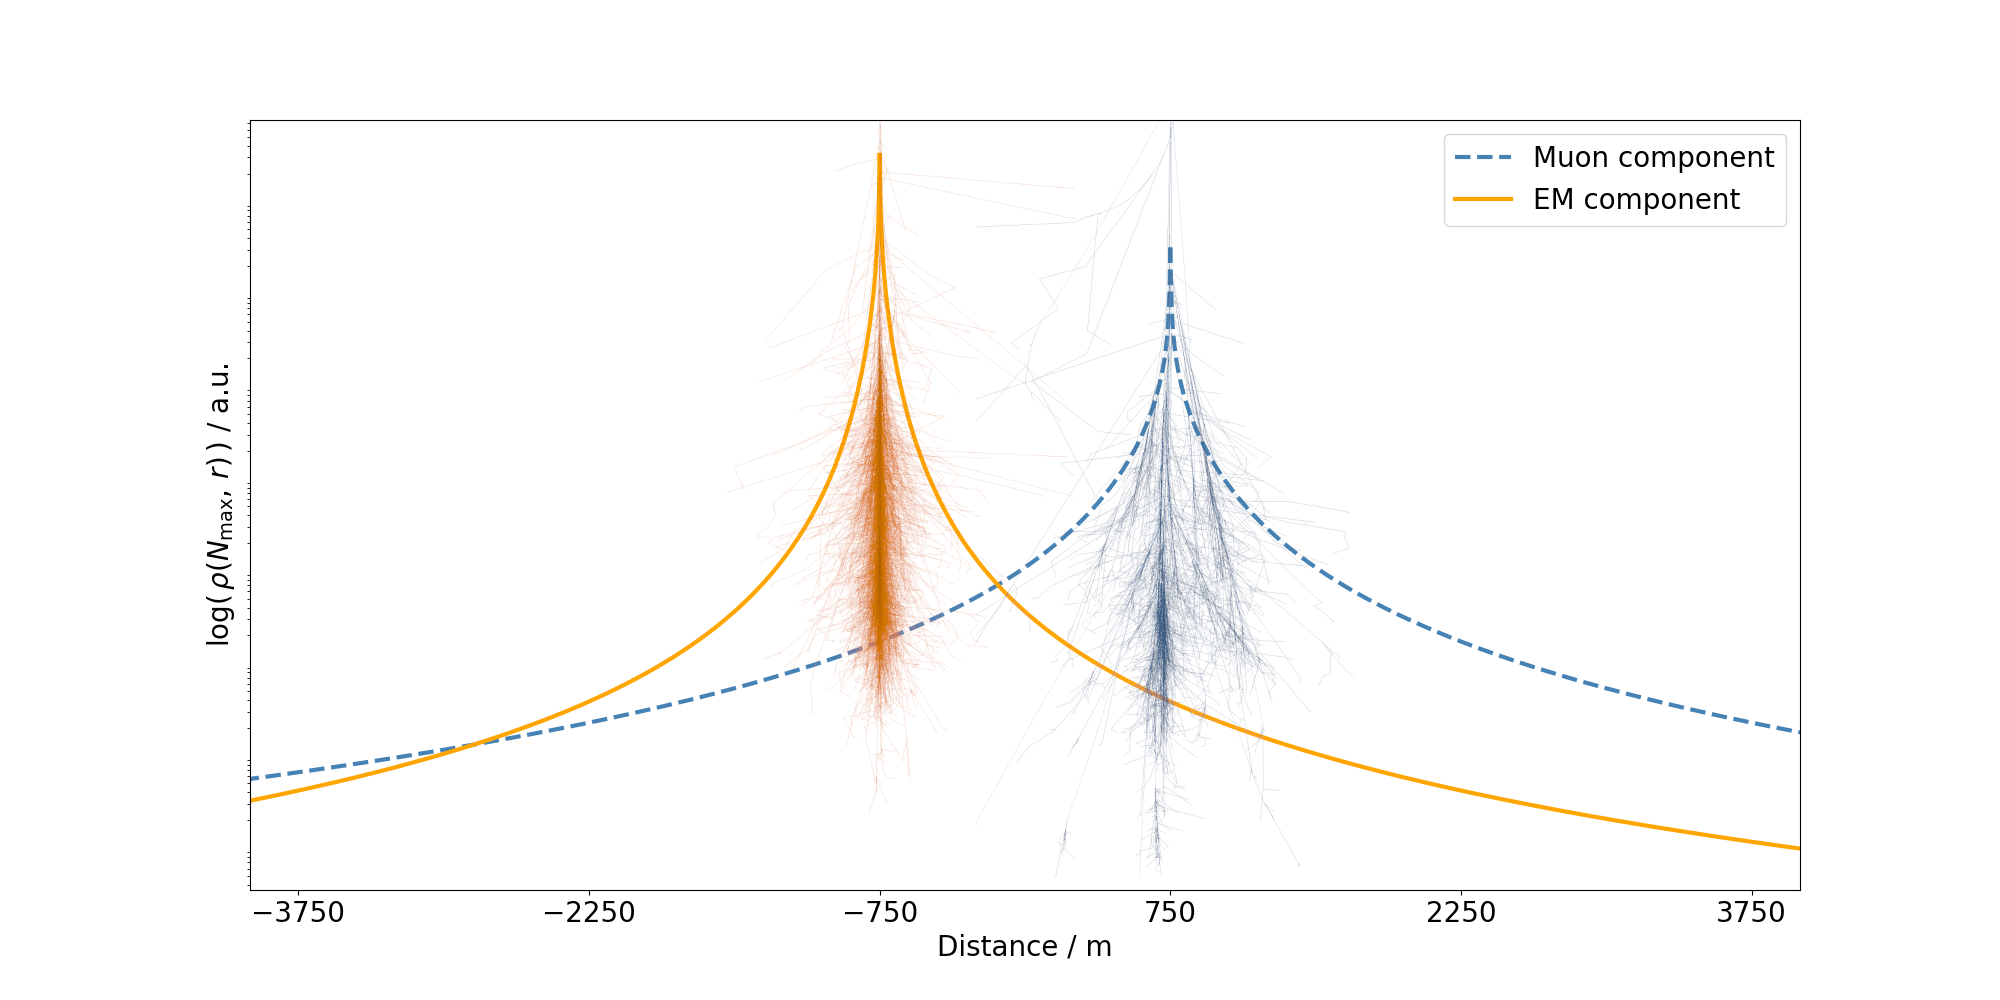
\includegraphics[width=1.0\textwidth]{./plots/componentwise_LDF.png}
	\caption{The lateral distribution function for the muonic (steelblue) and electromagnetic (orange) component of a vertical, \SI{100}{\giga\electronvolt}
	proton shower at roughly sea level ($r_\text{M}=\SI{100}{\meter}$). The inset plots represent the xz-projection of the color-coded shower component. Both 
	component images adopted with changes from \cite{CorsikaShower}.}
	\label{fig:component-LDF}
\end{figure}

\section{Composite primaries}
\label{sec:superposition-principle}

As is evident from the discussion in \autoref{chap:physical-background}, not only single protons (which are strictly speaking also composite) or elementary 
particles like photons, electrons, etc. appear in the cosmic ray spectrum. In theory, any somewhat stable particle is a possible primary. The consequence of 
different primaries on resulting shower characteristics is subtle, but large enough such that it can be used for identification purposes.

Assuming the constituents in a CR nucleus all coherently interact with an air molecule, one arrives at the superposition principle for extensive air showers. It 
states that for a composite primary with $A = N + Z$ neutrons and protons, each constituent particle will initiate a subshower with initial energy of 
$E_0' = E_0\,/\,A$, where $E_0$ is the initial energy of the composite particle. For this scenario, $N_\text{max}$ and $n_\text{max}$ are known from the preceding
sections. It follows that air showers from heaver primaries occur at higher altitudes (lower atmospheric depth $X$) and with higher particle counts.

\begin{equation}
N_{\text{max},\,A} = A \cdot N_{\text{max}}, \qquad n_{\text{max},\,A} = \left\lfloor \log_N\left(\frac{E_0}{E_{c,\,\text{had}}}\right) - \log_N A \right\rfloor,
\end{equation}

where $N_{\text{max},\,A}$, $n_{\text{max},\,A}$ refer to the resulting extensive air shower characteristics that are induced by a particle with mass number $A$.
On top of this, because more massive particles initiate more subshowers of comparably lower primary energy, and thus have lower $n_\text{max}$, less energy is 
transferred from the hadronic to the electromagnetic shower component. This results in differing fractions of muonic to electromagnetic signal in the shower 
footprint.

\section{Validity of shower simulations}
\label{sec:cr-shower-validity}

The Heitler model and Heitler-Matthews model discussed in \autoref{sec:heitler-model} and \autoref{sec:heitler-matthews-model} respectively make only very 
rudimentary assumptions on the underlaying physics of particle cascades. Nevertheless, the equations recovered from these assumptions are already a close 
approximation of real world processes up to $X_\text{max}$. 

Of course, adding a stochastic component to the above assumptions (c.f. \cite{MartinShowerSim}) improves predictions. But even full-fledged Monte-Carlo simulation 
software frameworks like GEANT4 \cite{agostinelli2003geant4} or CORSIKA \cite{heck1998corsika} show discrepancies between observed and predicted shower development
when analysed in depth. This is shown in \autoref{fig:model-validity}. 

While shower-to-shower fluctuations can explain discrepancies to a degree, there also exist systematic differences between the simulated and observed extensive air
showers. These are largely owed to imprecise knowledge of the underlaying physical processes. For example, hadronic interaction models (e.g. QGSJETII-04) rely on 
extrapolation of measured cross sections in the \SI{}{\giga\electronvolt}-\SI{}{\tera\electronvolt} scales to the relevant CR energies \cite{ostapchenko2006qgsjet}. 
While this is not an unfair assumption given the scale invariance of deep inelastic scattering \cite{fox1974early}, it is clear, that the approach cannot accurately 
encompass all effects that may take place at the high energies present in atmospheric particle cascades.

In conclusion, the particle cascades evolving from relativistic CRs impinging on earth are still not fully understood. Several simulation frameworks have been 
developed, which each have their own shortcomings. It is therefore important to compare not only results from simulations using one framework to observations, but 
also different simulations with each other.

\begin{figure}
	\centering
	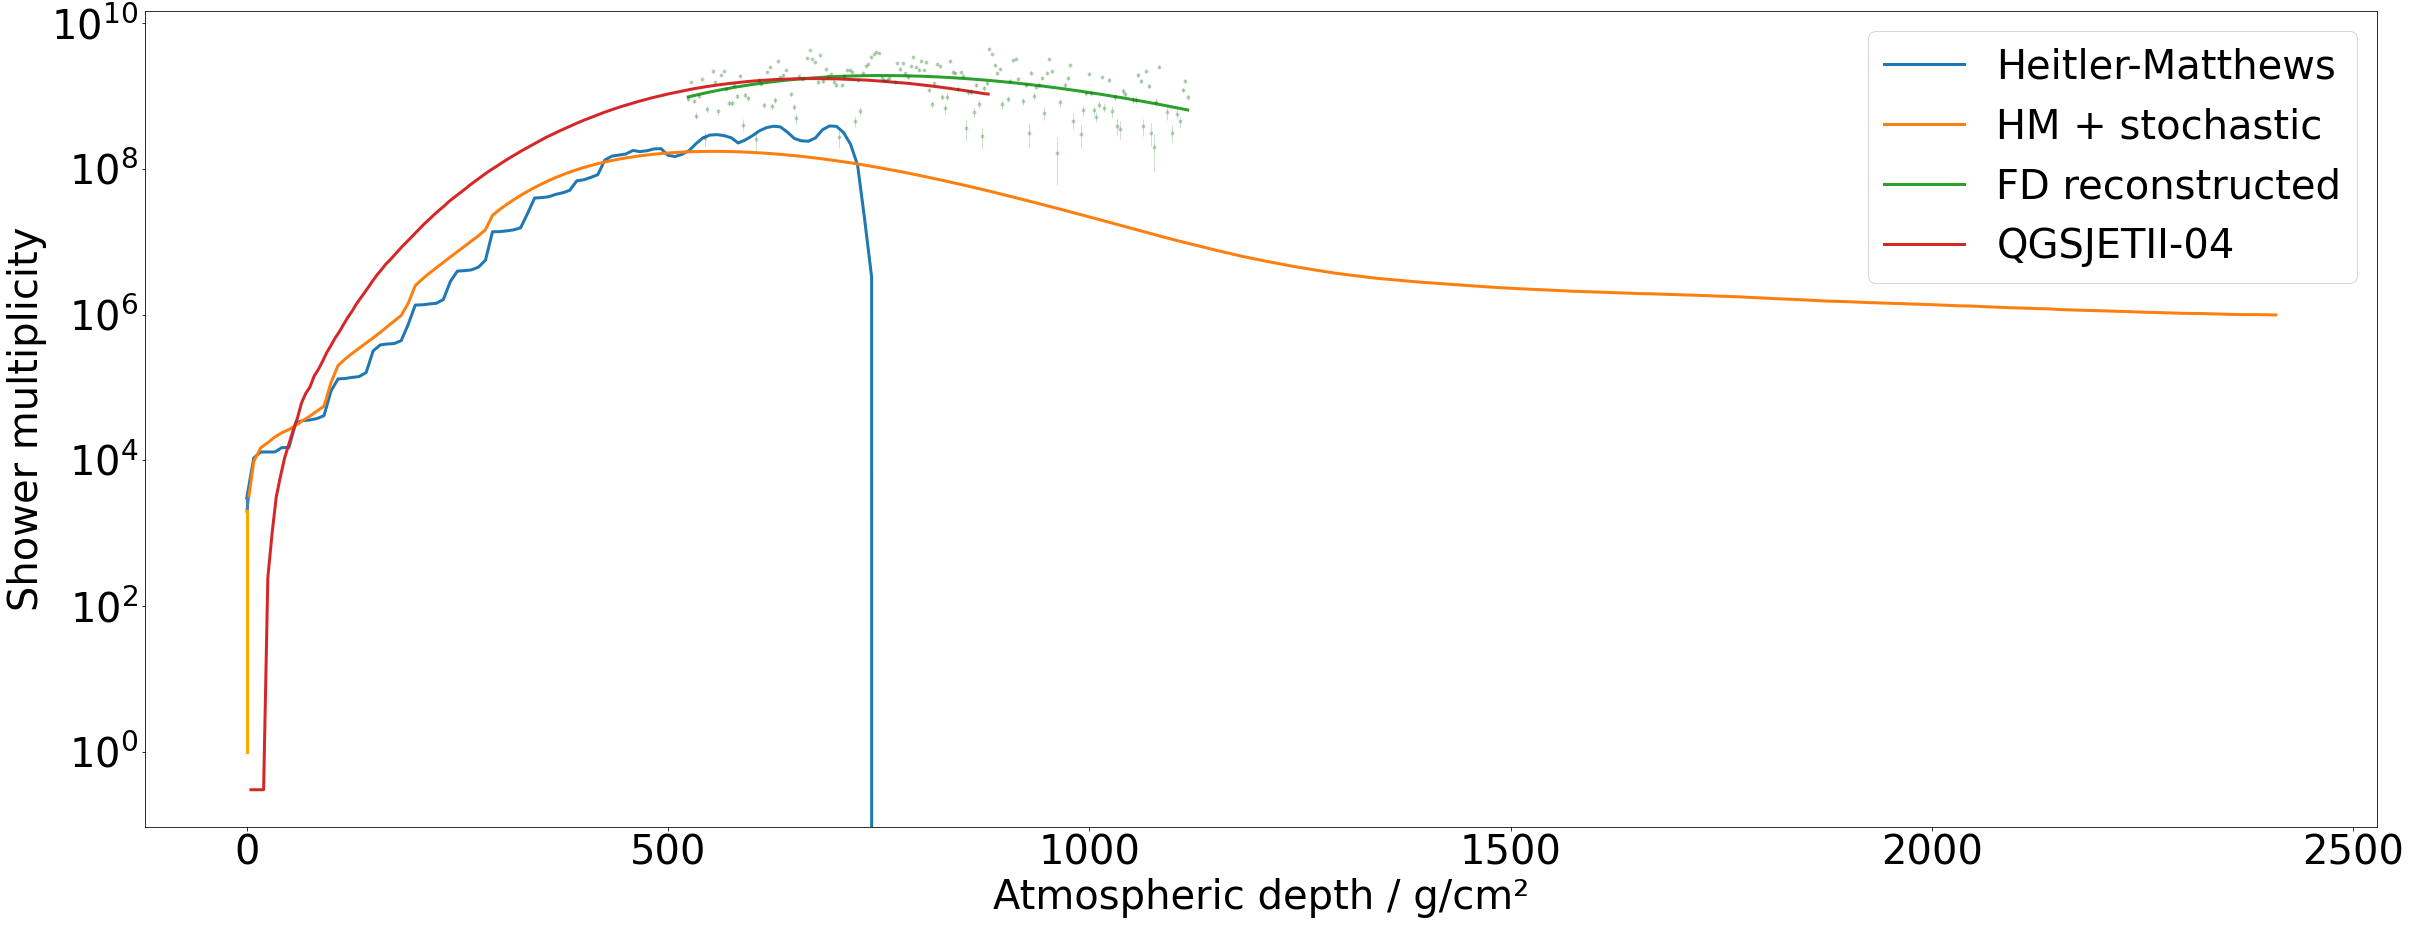
\includegraphics[width=1.0\textwidth]{./plots/validity_plot.png}
	\caption{Comparison of the number of charged particles for different physics models to reconstructed observations from a $~\SI{3}{\exa\electronvolt}$ proton 
	shower. Shown in steelblue and orange is the Heitler-Matthews model as described in \autoref{sec:heitler-matthews-model}, and extended with a stochastic 
	component. An example of a more in-depth simulation in red, and observed shower multiplicities in green.}
	\label{fig:model-validity}
\end{figure}

\section{Detection methods}
\label{sec:detection-methods}

\subsection{Cherenkov light}
\label{ssec:cherenkov-light}

When a charged particle exceeds the phase velocity of light in a medium with refractive index $n$, the optical equivalent of a sonic boom occurs. Photons travel in a 
shockwave along an angle $\theta = \arccos\left(n^{-1}\beta^{-1}\right)$ relative to the trajectory of the particle while $\beta \geq \frac{c}{n}$. This process is 
well understood and can be used to detect high energy cosmic rays.

\subsubsection{Imaging Air Cherenkov Telescope}

The refractive index of air ranges from 1 in the near vacuum of the upper atmosphere to $\approx1+2.9\cdot10^{-4}$ at sea level \cite{andrews1992analytical}. This
implies that particles with a Lorentz factor $\gamma \gtrsim 41.5$ emit Cherenkov light, which is satisfied for e.g. muons and protons in the low 
\SI{}{\giga\electronvolt} ranges and above.

It can therefore be expected that extensive air showers, which contain high energy charged particles, produce considerable amounts of Cherenkov light when 
propagating throught the atmosphere. This light, and by extension the air shower can be detected with \textbf{I}maging \textbf{A}ir \textbf{C}herenkov 
\textbf{T}elescopes (IACTs). Ground based experiments such as VERITAS \cite{VeritasTelescope} or H.E.S.S \cite{HessTelescope} detect gamma-rays using this technique.

\subsubsection{Water Cherenkov Detector}

The lightspeed in water is roughly $33\%$ slower than in vacuum. Cherenkov radiation in water therefore occurs more easily than in air. Using this reasoning, a 
water tank equipped with means of detecting the emitted Cherenkov light, via e.g. \textbf{P}hoto\textbf{M}ultiplier \textbf{T}ubes (PMTs), should be able to 
measure traces of an air shower. 

Indeed, this exact measurement principle of a \textbf{W}ater \textbf{C}herenkov \textbf{D}etector (WCD) was and is adopted in a variety of cosmic ray observatories 
such as the Pierre Auger observatory \cite{PierreAugerObservatory}, HAWC \cite{HAWC}, or Kamiokande \cite{Kamiokande}, for example.


\subsection{Fluoresence}
\label{ssec:fluoresence}

Ionization losses have been ignored in the discussion of the formation of extensive air showers. This is of course not completely accurate. During the development of 
an extensive air showers, particles excite, or even ionize the permeated medium. Consequently, spontaneous emission of photons due to recombination, or transition 
back to a ground state can be observed. The amount of fluorescence light produced in this way is a gauge for the number of particles present in the shower at a given
moment.

\subsubsection{In Air}

The predominant element in air is nitrogen ($78\%$), whose transitions lay in the UV-band \cite{FDReconstruction}. After a nitrogen molecule is excited by a passing
shower particle, a photon with wavelength $\SI{300}{\nano\meter} \leq \lambda \leq \SI{430}{\nano\meter}$ is emitted isotropically due to relaxation. The low 
attenuation of ultraviolet radiation in air allows the fluorescence light to travel large distances before being absorbed \cite{elterman1968uv}. This enables 
cameras like EUSO-TA \cite{abdellaoui2018euso} or the \textbf{F}lourescence \textbf{D}etector (FD) of the Pierre Auger observatory (see \cite{FDReconstruction} and
\autoref{sec:fluoresence-detector}) to observe traces of extensive air showers from faraway during their development. 

However, because of the low light yield of just \SI{5}{photons\per\MeV} \cite{nagano2004new}, the detectors must operate in low UV-noise conditions, which 
places an upper limit on their duty cycle.

\subsubsection{In Scintillators}

Conventional plastic scintillators have a light yield, that is $1000-10000$ times higher than that of air \cite{holl1988measurement}. Such scintillators therefore 
pose an effective way of measuring a shower footprint on the ground. The Pierre Auger \textbf{S}urface \textbf{D}etector (SD) is equipped with scintillators during
the ongoing AugerPrime upgrade. Predecessors like KASCADE \cite{Kascade} have been using scintillation light to detect cosmic rays as well.

\subsection{Radio Emission}
\label{ssec:radio-emission}

Relativistic charged particles in the cascade are subject to deflections due to the geomagnetic field. This deflection is largest for $e^\pm$ due to their 
comparably tiny masses. Albeit the deflection of a typical electron in the shower is miniscule and the subsequent emission of Bremsstrahlung tiny, coherence 
effects along the entire shower front can greatly amplify the electric field strengths obtained from this effect \cite{aab2018observation}. This gives rise to radio
signals emitted by the extensive air shower, which can in principle be detected via antennas.

One challenge in constructing an efficient CR radio detector is the requirement for a radio-quiet environment, where a large enough 
\textbf{S}ignal-to-\textbf{N}oise-\textbf{R}atio (SNR) permits analysis of measured data. This is the case for the AERA component of the Pierre Auger observatory,
which has been in operation since 2010 \cite{Aera}. Its results have in part lead the proposal of a vast radio array, GRAND \cite{Grand}, which will have an enormous 
exposure to CR showers, if built.
